\subsection{\large{\textit{oP}12-CuAsS (Direct)}}\vspace{-0.1in}
Lautite


\begin{figure}[H]
\begin{minipage}{0.34\textwidth}\centering
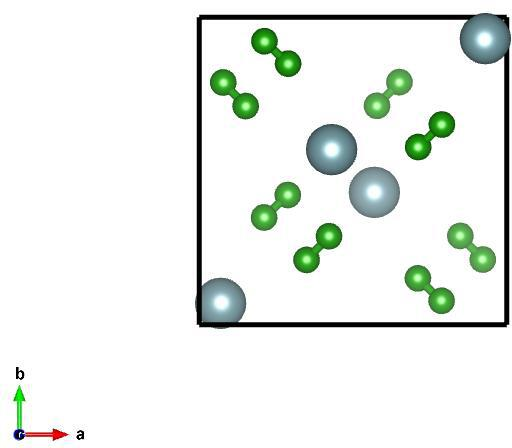
\includegraphics[width=0.9\linewidth,height=2in,keepaspectratio]{/Users/rosecers/work_folders/structures_for_photonics/reference/ref_inp/workspace/da2f2017abf551391169c27840af9313/final_images/analog_trim.jpg}\\
\small{Image of \textit{oP}12-CuAsS, generated by Vesta}
\end{minipage}\hfill
\begin{minipage}{0.65\textwidth}\raggedright
{\setlength{\mathindent}{0cm}
\begin{equation*}
\begin{split}&\boldsymbol{a_1} = \ \hat{x}\\[-8pt]
&\boldsymbol{a_2} = 0.3307746463\ \hat{y}\\[-8pt]
&\boldsymbol{a_3} = 0.4805675518\ \hat{z}
\end{split}
\end{equation*}}

\textbf{Space Group:}	62\hspace{0.5in}\textbf{Point Group:}	$mmm$\\
\textbf{Crystallographic Open Database} \#2217766\\
\textbf{Structure DOI: }\url{10.1107/S1600536808004492}

\end{minipage}\hfill
\end{figure}
\vspace{-0.25in}


\begin{figure}[H]
\begin{minipage}{0.9\textwidth}\centering
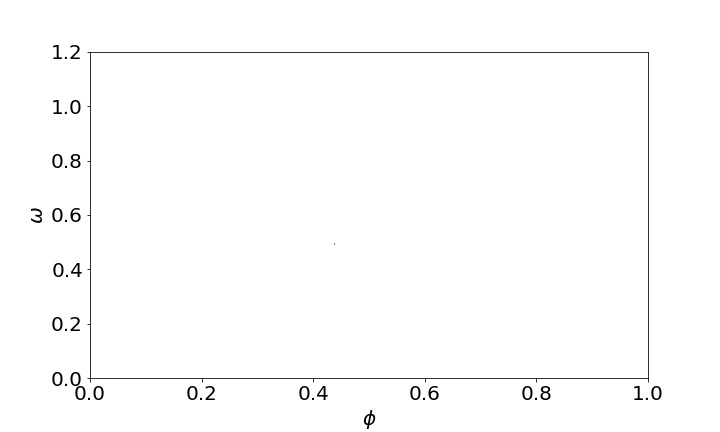
\includegraphics[width=0.9\linewidth,height=2.5in,keepaspectratio]{/Users/rosecers/work_folders/structures_for_photonics/reference/ref_inp/workspace/da2f2017abf551391169c27840af9313/final_images/gap_atlas.jpg}
\\
\end{minipage}\hfill\caption{Gap Atlas across filling fraction $\phi$ and frequency $\omega$}
\end{figure}


\begin{figure}[H]
\begin{minipage}{0.5\textwidth}\centering
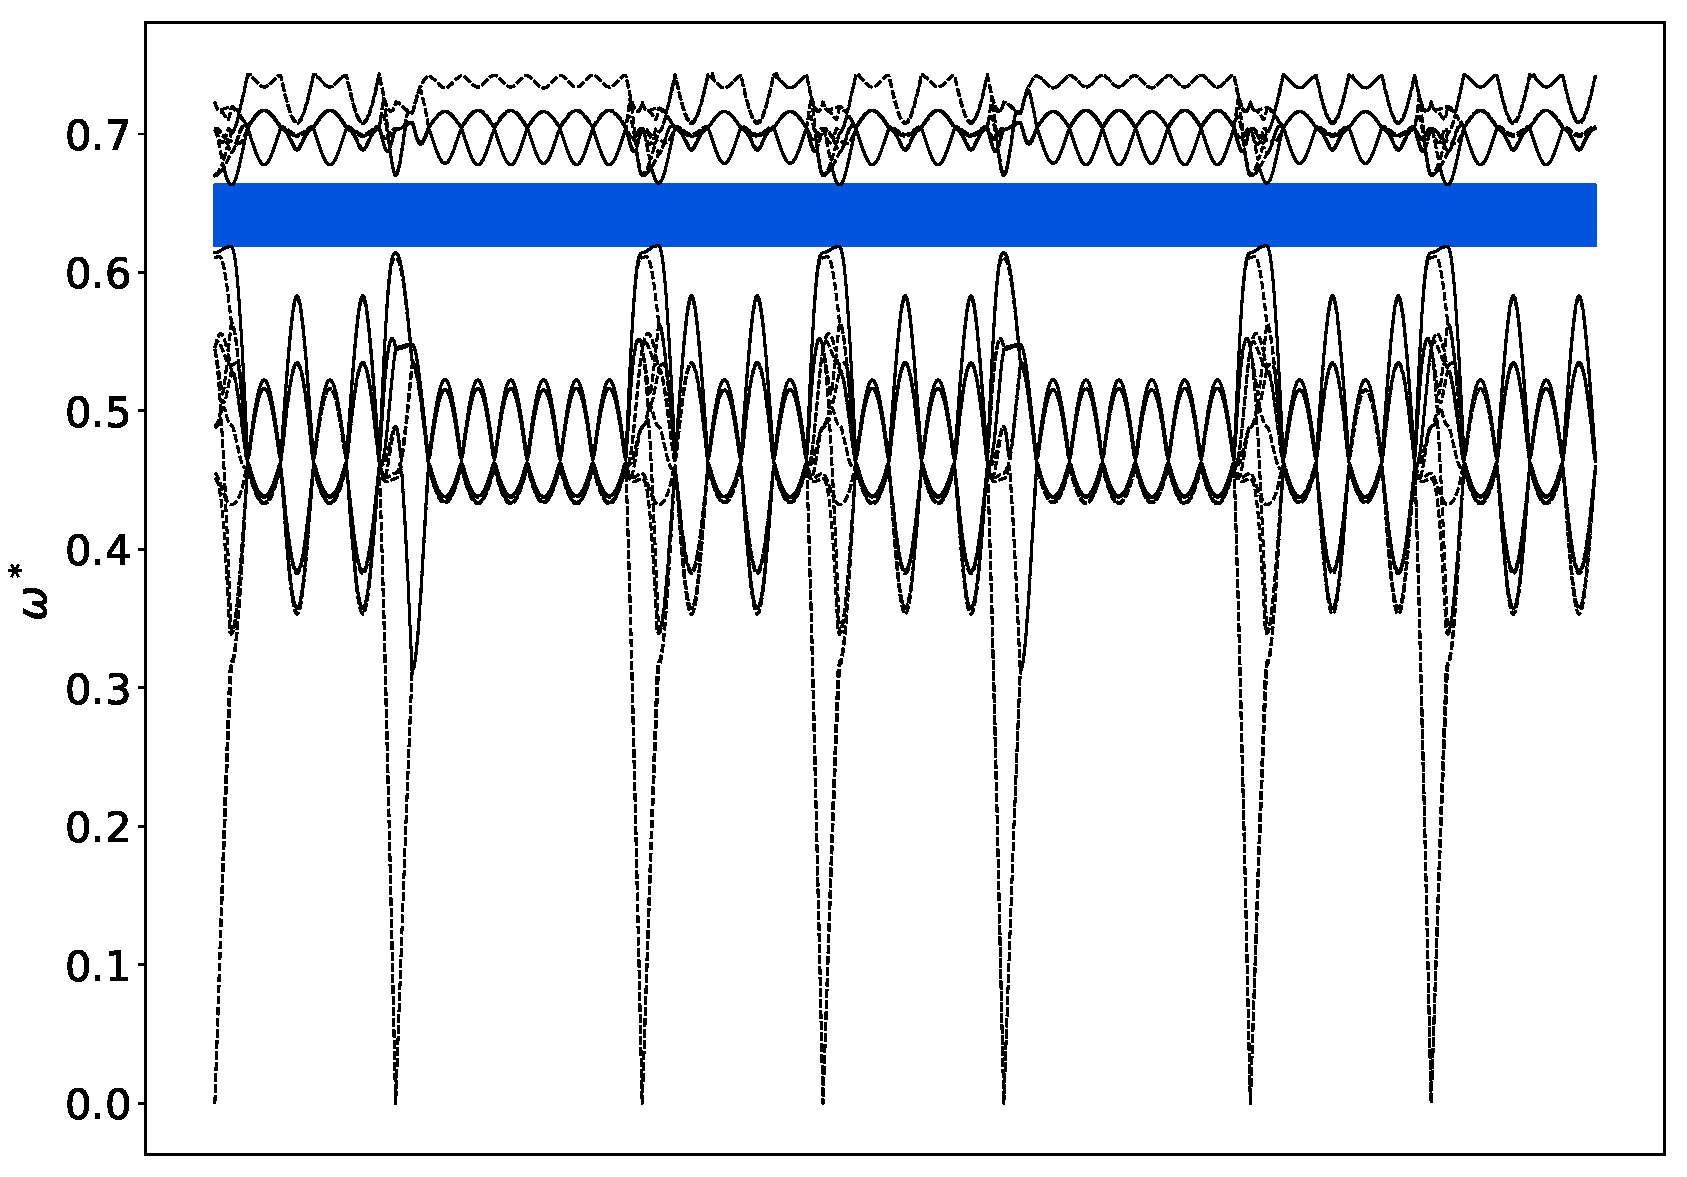
\includegraphics[width=0.9\linewidth,height=1.5in,keepaspectratio]{/Users/rosecers/work_folders/structures_for_photonics/reference/ref_inp/workspace/da2f2017abf551391169c27840af9313/./final_images/band_diagram_b=12.pdf}
\\Band Structure across 1st BZ
\end{minipage}\hfill
\begin{minipage}{0.48\textwidth}\centering
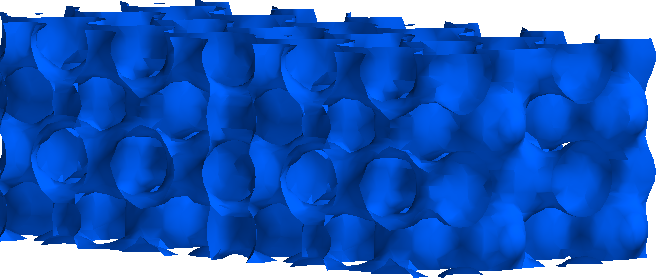
\includegraphics[width=0.9\linewidth,height=1.5in,keepaspectratio]{/Users/rosecers/work_folders/structures_for_photonics/reference/ref_inp/workspace/da2f2017abf551391169c27840af9313/final_images/oP12-CuAsS@gap_12-13.png}
\\View along $a_1$ 
\end{minipage}\hfill\caption{Band Structure and Isosurface of \textit{oP}12-CuAsS (Direct) at radius = 0.12, filling fraction = 0.514, where the largest gap between bands 12 and 13 occurs with gap size 10.0\%.}

\end{figure}
\vspace{-0.25in}

